\begin{frame}
    \frametitle{Site Yahoo! Finance}
    
    	   \begin{figure}[H]
      \center
      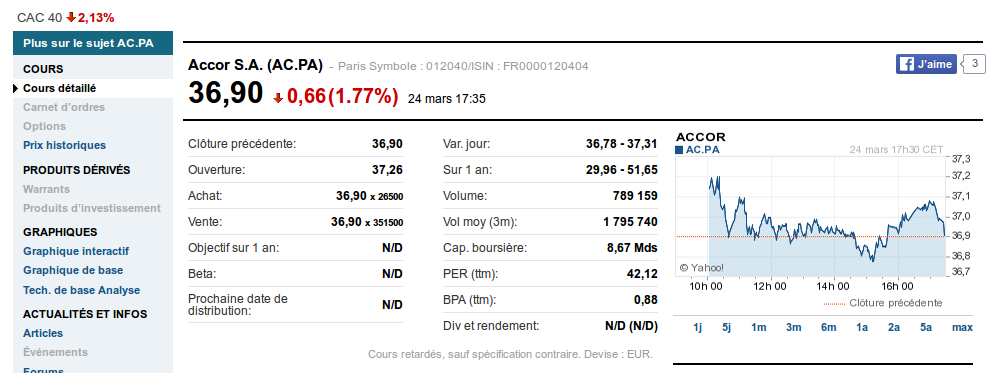
\includegraphics[scale=0.30]{images/yahoo.png}
      \caption{Visualisation du site Yahoo! Finance pour l'action ACCOR S.A}
      \end{figure}
    	   
\end{frame}

\begin{frame}[fragile]
    \frametitle{Principe du téléchargement}
    \begin{block}{Code JAVA}
  \begin{lstlisting}[language=JAVA, basicstyle=\scriptsize] 
String url="http://real-chart.finance.yahoo.com/table.csv?"+
	"s="+code  
	+"&a="+debut.get(Calendar.MONTH) 
	+"&b="+debut.get(Calendar.DAY_OF_MONTH) 
	+"&c="+debut.get(Calendar.YEAR) 
	+"&d="+fin.get(Calendar.MONTH)
	+"&e="+fin.get(Calendar.DAY_OF_MONTH)
	+"&f="+fin.get(Calendar.YEAR)
	+"&g=d" 
	+"&ignore=.csv"; 
\end{lstlisting}	  
	\end{block}

\end{frame}
